\chapter{РАЗРАБОТКА ПРОГРАММЫ ДЛЯ ГЕНЕРАЦИИ СИГНАЛОВ}
\section{Моделирование DDS}
	Для начала потребуется таблица отсчётов, чтобы её вычислить используем готовый инструмент~\cite{lut}.
	
%	\begin{figure}[H]
%    \centering
%    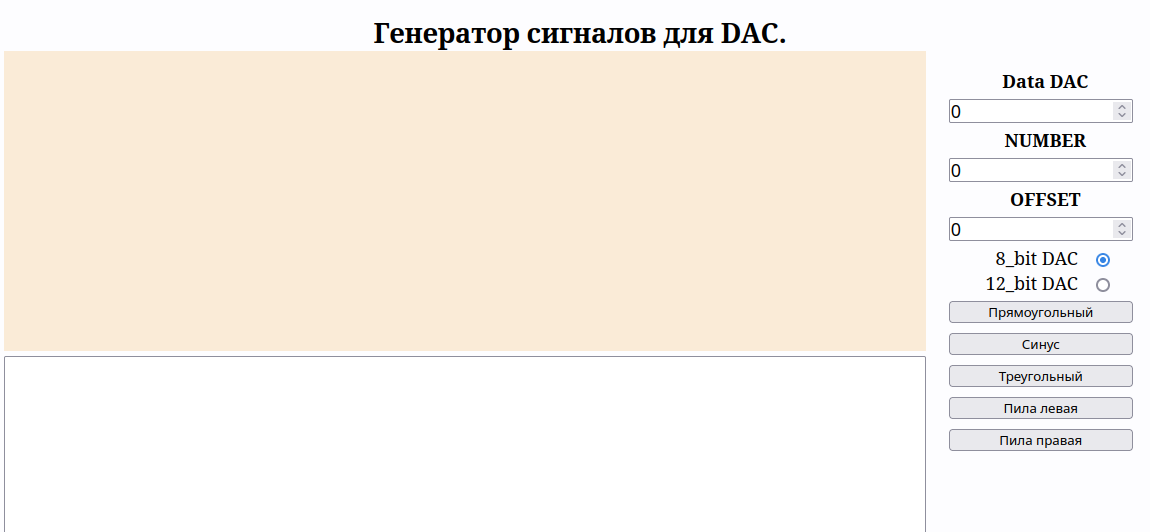
\includegraphics[width=1\textwidth]{../image/lut_prog.png}
%    \caption{Программа для вычисления значений сигнала.}
%	\end{figure}
	
	У таблицы есть 5 параметров:
	\begin{enumerate}
		\item Максимальное значение;
		\item Количество значений;
		\item Смещение от нуля;
		\item Разрядность ЦАП: 8 или 12 бит;
		\item Форма сигнала.
	\end{enumerate}
	
	В данной работе будут использоваться 12-битные значения в количестве 256 чисел. Максимальное значение амплитуды сигнала может быть 4095. Для примера вычислим таблицу значений для синусоиды.
	
	\begin{figure}[H]
    \centering
    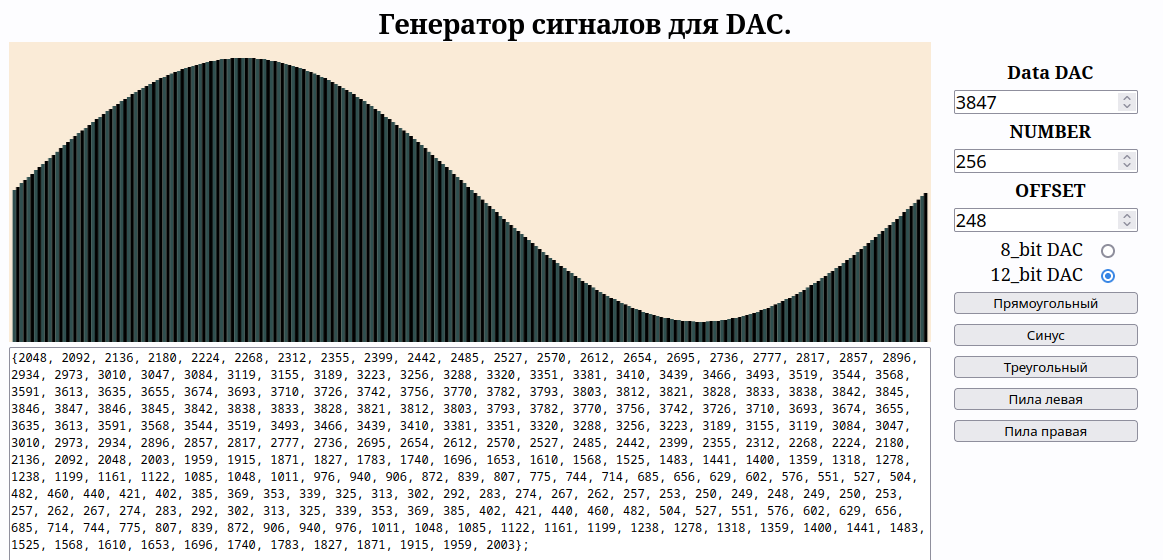
\includegraphics[width=1\textwidth]{../image/lut.png}
    \caption{Вычисление таблицы сигнала.}
	\end{figure}
	
	Теперь у нас есть данные для генерации сигнала. Смоделируем алгоритм метода прямого цифрового синтеза по блок-схеме на рис. 1.15 на языке Си для дальнейшей реализации на микроконтроллере.

\begin{code}
\captionof{listing}{Метод DDS}
\begin{minted}[mathescape,linenos,frame=lines,breaklines]{text}
int main() {
  uint16_t p_acc, p_step;
  uint8_t addr = 0; // адрес ячейки

  p_acc = 0;    // аккумулятор фазы
  p_step = 128; // код частоты

  while(1) {
    addr = p_acc >> 8; // выделение старшей части аккумулятора фазы
    p_acc += p_step;   // шаг
    printf("%d 0x%X\n", addr, sinus[addr]); // вывод отсчёта
  }

  return 0;
}
\end{minted}
\end{code}

	
	Код частоты задаёт выходную частоту генератора. При значении 256 вывод будет следующий:
	
\begin{figure}[H]
    \centering
    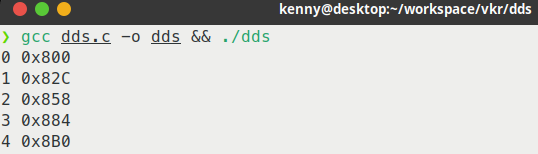
\includegraphics[width=0.6\textwidth]{../image/dds256.png}
    \caption{Формирование отсчётов при коде частоты 256.}
\end{figure}
	
	Увеличим код частоты в два раза и получим следующее:

\begin{figure}[H]
    \centering
    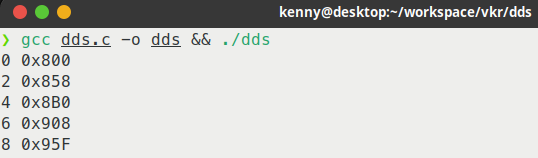
\includegraphics[width=0.6\textwidth]{../image/dds512.png}
    \caption{Формирование отсчётов при коде частоты 512.}
\end{figure}

	Как можно заметить отсчёты стали формироваться через один, соответственно частота вырастит в два раза. Теперь уменьшим частоту в два раза выставив код частоты 128.

\begin{figure}[H]
    \centering
    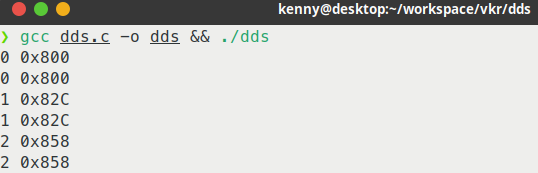
\includegraphics[width=0.6\textwidth]{../image/dds128.png}
    \caption{Формирование отсчётов при коде частоты 128.}
\end{figure}

	Программа стала выводить каждый отсчёт по два раза тем самым, понизив частоту.
	
	В данном виде модуляции код частоты просто абстрактное число, которое добавляется к аккумулятору фазы и узнать реальную частоту проблематично. Результат синтеза будет проверен опытным путём на микроконтроллере.
	
\section{Обзор микроконтроллеров}
	Так как генератор сигналов будет реализовываться на микроконтроллере следует провести обзор и осуществить выбор. Рассмотрим два популярных семейства микроконтроллеров AVR и STM32.
\subsection{AVR}
	Микроконтроллеры AVR --- это 8-разрядные микроконтроллеры с архитектурой RISC. Данное семейство представляет собой хорошую основу для создания высокопроизводительных и экономичных встраиваемых систем~\cite{avrstm}. Подразделяется семейство на две группы: Tiny и Mega.
	
	Микроконтроллеры Tiny имеют небольшую память для программ и их периферия ограничена. Большинство микроконтроллеров данной серии выпускаются в 8-выводных корпусах и предназначены для систем с ограниченным бюджетом. Областью их применения являются различные датчики и бытовая техника~\cite{avr}.
	
	Группа Mega наоборот имеет большую память и развитую периферию. Соответственно область применения гораздо шире и предназначены они для более сложных систем. В таблице 2.1 приведены серии микроконтроллеров и коротко описан их приоритет.

\begin{table}[H]
\caption{Микроконтроллеры AVR}
\begin{tabular}{|p{3.25 cm}|p{8 cm}|p{4 cm}|}
\hline
Группа & Приоритет & Название серий \\ \hline
Tiny & Энергоэффективность, компактность, низкая стоимость & tiny1, tiny2, tiny4, tiny8 \\ \hline
Mega & Производительность, гибкость & mega4, mega8, mega16, mega32, mega64, mega128, mega256 \\ \hline
\end{tabular}
\end{table}

\subsection{STM32}
	Микроконтроллеры STM32 --- это 32-разрядные микроконтроллеры, имеющие процессорное ядро с архитектурой ARM Cortex-M. В настоящее время существует множество микроконтроллеров STM32. Они делятся на семейства в зависимости от версии архитектуры (табл. 2.2).

\begin{table}[H]
\caption{Семейства STM32}
\begin{tabular}{|p{4 cm}|p{4 cm}|}
\hline
Серия & Ядро \\ \hline
F0  & Cortex-М0 \\ \hline
G0, L0  & Cortex-М0+ \\ \hline
F1, F2  & Cortex-М3 \\ \hline
F3, F4, L4, G4  & Cortex-М4 \\ \hline
F7, H7  & Cortex-М7 \\ \hline
\end{tabular}
\end{table}

	Ядро Cortex-M обеспечивает программную совместимость во всех семействах. Кроме этого, для микроконтроллеров выпущенных в одинаковых корпусах присутствует и аппаратная совместимость, так как на выводах сохраняются одни и те же функции~\cite{stm, avrstm}. Будем рассматривать серии микроконтроллеров схожие по функциональным возможностям с Tiny и Mega для дальнейшего сравнения. В таблице 2.3 указаны серии STM32 по группам.
	
\begin{table}[H]
\caption{Микроконтроллеры STM32}
\begin{tabular}{|p{3.25 cm}|p{8 cm}|p{4 cm}|}
\hline
Группа & Приоритет & Название серий \\ \hline
Широкого применения & Баланс между производительностью и энергоэффективностью & F0, G0, F1, F3,
G4 \\ \hline
Сверхнизкого энергопотребления & Энергоэффективность, компактность, низкая стоимость & L0, L4 \\ \hline
\end{tabular}
\end{table}

\section{Сравнение семейств AVR и STM32}
	
	Для осуществления выбора проведём сравнение микроконтроллеров, взяв параметры наиболее используемых серий из каждой группы (табл. 2.4). Параметры получены из спецификаций на микроконтроллеры ~\cite{f103,l1010f4,atmega32,attiny10}.
	
\begin{table}[H]
\caption{Параметры микроконтроллеров}
\begin{tabular}{|p{2.5 cm}|p{3 cm}|p{3 cm}|p{3.1 cm}|p{3.1 cm}|}
\hline
        Параметр & ATtiny10 & ATmega32 & STM32L010F4 & STM32F103xC \\ \hline
        Частота & 20 МГц & 20 МГц & 32 МГц & 72 МГц \\ \hline
        FLASH & 1 Кбайт & 32 Кбайт & 16 Кбайт & 256 Кбайт \\ \hline
        RAM & 64 байт & 2 Кбайт & 2 Кбайт & 48 Кбайт \\ \hline
        SPI & - & + & + & + \\ \hline
        I2C & - & +	 & + & + \\ \hline
        Питание & 1,8 --- 5,5 В & 1,8 --- 5,5 В & 1,8 --- 3,6 В & 1,8 --- 3,6 В \\ \hline
\end{tabular}
\end{table}
	
	Исходя из таблицы можно сделать вывод, что микроконтроллеры AVR применимы в малом спектре задач где скорость не так важна. В нашем же случае скорость работы микроконтроллера может сильно влиять на генерацию сигнала, а также требуется объём памяти для хранения отсчётов сигналов. В микроконтроллерах STM32 с частотой и объёмом памяти проблем нет и они имеют широкое применение. Серию же выберем F103xC за её характеристики. В связи с этим, а также доступностью отладочных плат будет применён микроконтроллер STM32F103RCT6.

\section{Среды разработки для STM32}

	Среда разработки является не маловажным инструментом для создания программной части устройства. В связи с выбором микроконтроллера STM32 рассмотрим популярные бесплатные среды для создания программы на этом семействе микроконтроллеров.

\subsection{STM32CubeIDE}

	
	STM32CubeIDE --- это продвинутая платформа разработки на C/C++ с функциями настройки периферийных устройств, генерации кода, компиляции кода и отладки для микроконтроллеров и микропроцессоров STM32~\cite{cube}. Среда разработки основана на платформе Eclipse и GCC toolchain для разработки и GDB для отладки. Она позволяет интегрировать сотни существующих плагинов, которые дополняют возможности Eclipse IDE. Имеет расширенные функции отладки, включая: просмотр ядра ЦП, регистров периферийных устройств и памяти, анализ системы просмотра переменных в режиме реального времени. Поддерживается на операционных системах: Linux, macOS, Windows.
	
	\begin{figure}[h]
    \centering
    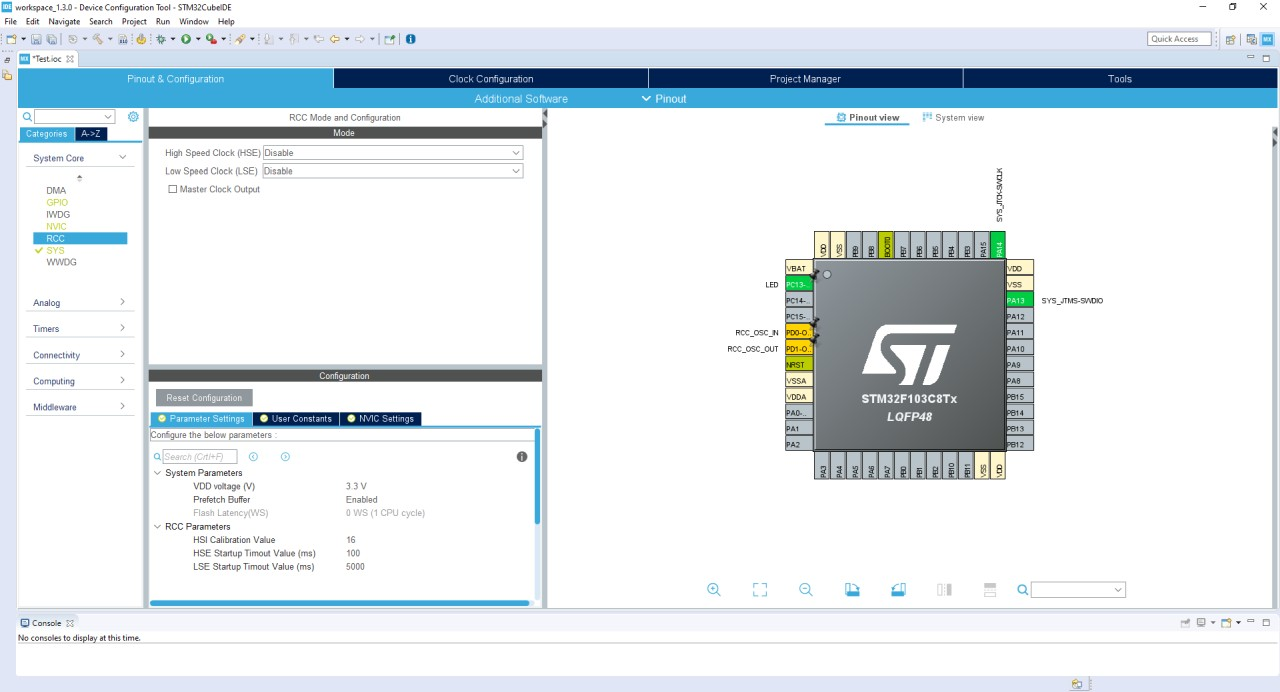
\includegraphics[width=0.9\textwidth]{../image/cube.jpg}
    \caption{Интерфейс STM32CubeIDE.}
	\end{figure}
	
	После выбора микроконтроллера STM32 создается проект и генерируется код инициализации. В любой момент разработки пользователь может вернуться к инициализации и настройке периферийных устройств и повторно создать код инициализации без какого-либо влияния на пользовательский код. Для разработки используется библиотека HAL. 
	
	Драйверы HAL включают в себя полный набор готовых к использованию функций, которые упрощают реализацию пользовательских приложений. Например, коммуникационные периферийные устройства содержат функции для инициализации и настройки периферийного устройства, управления передачей данных, обработки прерываний или DMA~\cite{hal}.
	
	Достоинства:
	\begin{itemize}
		\item поддержка различных ОС;
		\item расширенные возможности отладки;
		\item большое сообщество;
		\item автогенерация кода.
	\end{itemize}
	
	Недостатки:
	\begin{itemize}
		\item требовательность к ресурсам ПК;
		\item сложность настройки.
	\end{itemize}

\subsection{PlatformIO}

	PlatformIO --- удобная и расширяемая интегрированная среда разработки с набором профессиональных инструментов разработки, предоставляющая современные и мощные функции для ускорения и упрощения процесса разработки встраиваемых продуктов~\cite{plio}.
	
	\begin{figure}[h]
    \centering
    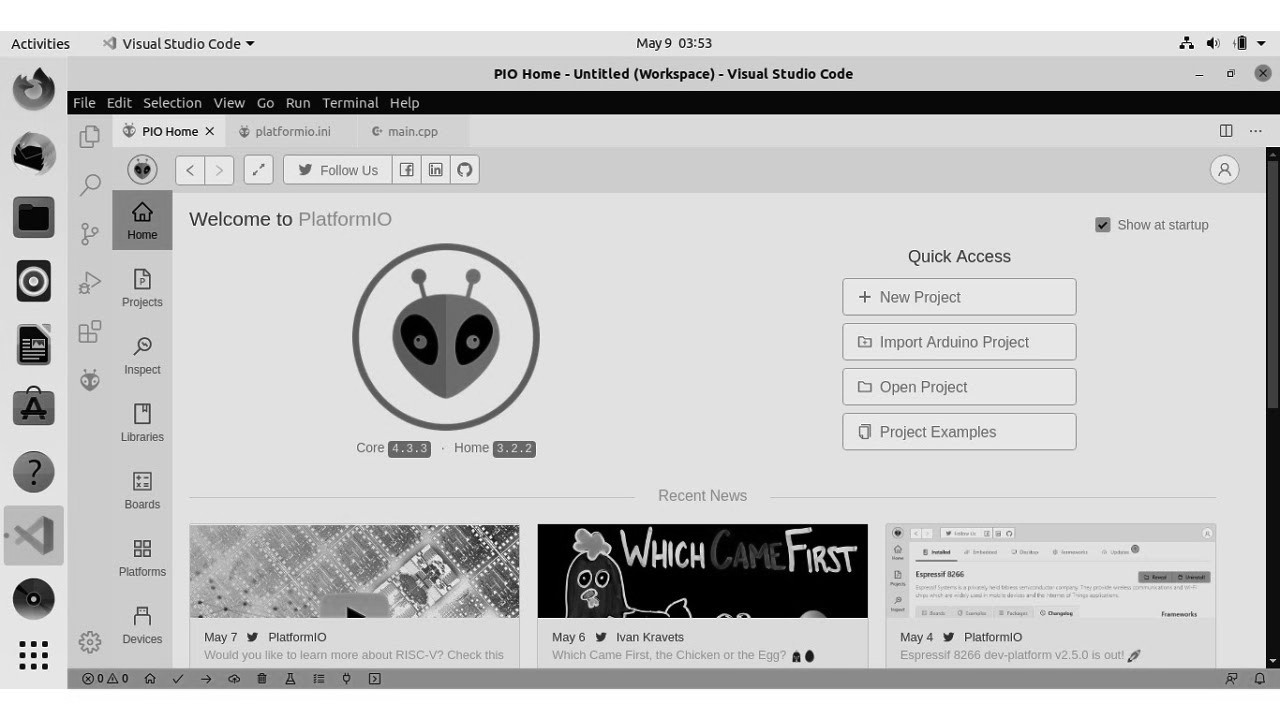
\includegraphics[width=0.9\textwidth]{../image/plio.jpg}
    \caption{Интерфейс PlatformIO.}
	\end{figure}
	
	Данная среда разработки является расширением для текстового редактора Visual Studio Code. VS Code --- это легкий, но мощный редактор кода, имеющий богатую экосистему расширений~\cite{vscode}. Доступен для Windows, macOS и Linux. Работа в паре с VS Code позволяет удобно форматировать код и пользоваться расширениями для языков программирования.
	
	PlatformIO позволяет работать со многими микроконтроллерами и поддерживает множество фреймворков для них, а также библиотек~\cite{docsplio}. Ввиду такой широкой поддержки, для STM32 можно разрабатывать с удобной для себя библиотекой. Это может быть к примеру тот же HAL, что и в STM32CubeIDE или libopencm3. Проект libopencm3 (ранее известный как libopenstm32) направлен на создание бесплатной библиотеки микропрограмм с открытым исходным кодом (LGPL версии 3 или более поздней) для различных микроконтроллеров ARM Cortex-M3, включая ST STM32~\cite{lcm3}.


	Достоинства:
	\begin{itemize}
		\item поддержка различных ОС;
		\item быстрая компиляция;
		\item поддержка GitHub;
		\item возможность работать с разными фрэймворками и платформами.
	\end{itemize}
	
	Недостатки:
	\begin{itemize}
		\item высокий порог вхождения;
		\item сложность установки.
	\end{itemize}

	Попользовавшись обеими средами разработки и разными библиотеками, а также основываясь на достоинствах и недостатках была выбрана среда разработки PlatformIO в связке с библиотекой libopencm3, использующая язык программирования Си~\cite{ckd, cdh}.


\section{Алгоритм работы программы для генерации сигналов}

	Структурно устройство будет выглядеть следующим образом (рис. 2.8). Цифро-аналоговый преобразователь будет использоваться встроенный в микроконтроллер, а в качестве дисплея будет выступать OLED экран с разрешением 128 на 64 пикселя, работающий по интерфейсу I2C на контроллере SSD1306.
	
	\begin{figure}[H]
    \centering
    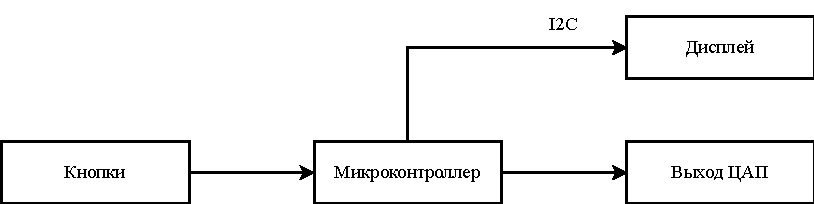
\includegraphics[width=1\textwidth]{../image/struct_gen.pdf}
    \caption{Структурная схема генератора сигналов.}
	\end{figure}
	
	Дисплей понадобится для вывода информации о форме сигнала, частоте и шаге регулировки частоты. Кнопки будут подключены напрямую к микроконтроллеру в количестве пяти штук для выполнения действий:
	\begin{enumerate}
		\item Уменьшить частоту;
		\item Увеличить частоту;
		\item Предыдущий сигнал;
		\item Следующий сигнал;
		\item Выбор шага.
	\end{enumerate}

	Программа должна выполнять три действия:
	
	\begin{enumerate}
		\item Вывод отсчёта в ЦАП (генерация сигнала);
		\item Обработка кнопок;
		\item Вывод информации на дисплей.
	\end{enumerate}
	
	
	Для цифро-аналогового преобразователя и кнопок выделим два таймера общего назначения. Таймер номер два будет использоваться для ЦАПа, а номер три для обработки кнопок. На примере третьего таймера рассмотрим его настройку. Алгоритм следующий:
	
	\begin{enumerate}
		\item Включить тактирование таймера;
		\item Задать стартовое значение;
		\item Установить предделитель;
		\item Установить период таймера;
		\item Включить прерывания от таймера;
		\item Запустить таймер.
	\end{enumerate}	 
	
	Кроме этого потребуется активировать прерывания и установить им приоритеты.
	
	Таймеры относятся к периферийным устройствам, а вся внутренняя периферия STM32 тактируется от шин APB1 и APB2 (Advanced Peripheral Bus)~\cite{tim}. В нашем случае таймеры тактируются от шины APB1, частота которой составляет 36 МГц~\cite{f103}. От предделителя зависит количество отсчётов таймера в секунду. Следовательно, если выставить предделитель 36000 получим следующее:
	
	\begin{center}
	$\dfrac{36*10^{6}}{36*10^{3}}=1000.$
	\end{center}
	
	Таймер будет делать 1000 отсчётов в секунду. Таким образом, 1 отсчёт таймера будет равняться 1 миллисекунде реального времени. Выставив период 250 получим прерывание от таймера каждые 250 мс. Данного времени хватит для обработки нажатия кнопки, тем самым решается проблема дребезга кнопок без использования программных или аппаратных задержек.
	
\begin{code}
\captionof{listing}{Настройка таймеров и прерываний}
\begin{minted}[mathescape,linenos,frame=lines,breaklines]{text}
static void timers_setup(void)
{
    rcc_periph_clock_enable(RCC_TIM2);
    rcc_periph_clock_enable(RCC_TIM3);

    /* Стартовое значение таймера */
    TIM_CNT(TIM2) = 0;
    TIM_CNT(TIM3) = 0;

    /* Предделитель 36MHz/36000 => 1000 отсчетов в секунду (счет начинается с 0, поэтому в предделителе и периоде нужно отнимать единичку) */
    TIM_PSC(TIM2) = 17;
    TIM_PSC(TIM3) = 35999;

    /* Период таймера */
    TIM_ARR(TIM2) = 9;
    TIM_ARR(TIM3) = 249;

    /* Включить прерывания */
    TIM_DIER(TIM2) |= TIM_DIER_UIE;
    TIM_DIER(TIM3) |= TIM_DIER_UIE;

    /* Запустить таймер */
    TIM_CR1(TIM2) |= TIM_CR1_CEN;
    TIM_CR1(TIM3) |= TIM_CR1_CEN;
}

static void nvic_setup(void)
{
    /* Активировать прерывания и установить приоритеты */
    nvic_enable_irq(NVIC_TIM2_IRQ);
    nvic_set_priority(NVIC_TIM2_IRQ, 2);

    nvic_enable_irq(NVIC_TIM3_IRQ);
    nvic_set_priority(NVIC_TIM3_IRQ, 1);
}
\end{minted}
\end{code}

	
	Таким образом, подпрограмма обработки кнопок будет размещена в обработчике прерывания от третьего таймера и будет состоять из функций для каждой кнопки.
	
	
\begin{code}
\captionof{listing}{Обработка кнопок}
\begin{minted}[mathescape,linenos,frame=lines,breaklines]{text}
void tim3_isr(void) // обработчик прерывания таймера3 (обработка кнопок)
{
    minus_freq();
    plus_freq();
    minus_signal(); // функции кнопок
    plus_signal();
    step_select();
    TIM_SR(TIM3) &= ~TIM_SR_UIF; // очистка флага прерывания
}
\end{minted}
\end{code}

	Обработка кнопок представлена следующей блок-схемой.	
	
	\begin{figure}[H]
    \centering
    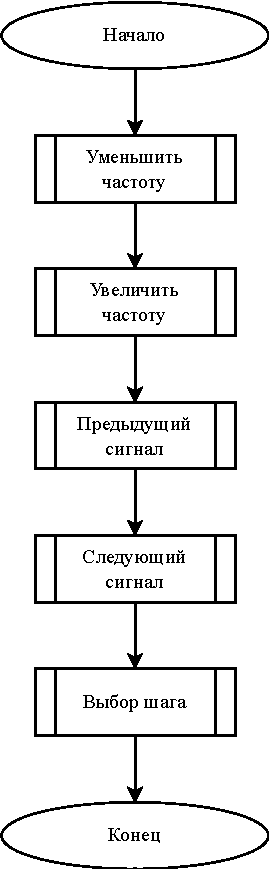
\includegraphics[width=0.3\textwidth]{../image/buttons.pdf}
    \caption{Блок-схема алгоритма функции кнопок.}
	\end{figure}
	
	Подпрограмма для вывода отсчёта в ЦАП будет размещена в обработчике прерывания второго таймера
	
\begin{code}
\captionof{listing}{Генерация сигнала}
\begin{minted}[mathescape,linenos,frame=lines,breaklines]{text}
void tim2_isr(void) // обработчик прерывания таймера2 (ЦАП)
{
    dac_load_data_buffer_single(signal[p_acc >> 8], RIGHT12, CHANNEL_2); // загрузка буфера в цап
    p_acc += p_step;             // шаг
    TIM_SR(TIM2) &= ~TIM_SR_UIF; // очистка флага прерывания
}
\end{minted}
\end{code}

	Работу подпрограммы генерации сигнала описывает следующая блок-схема.
	
	\begin{figure}[H]
    \centering
    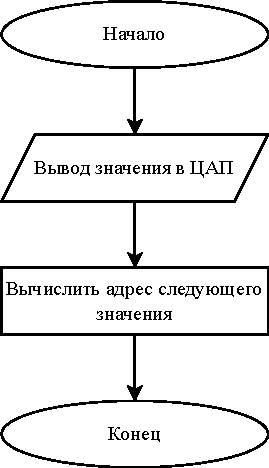
\includegraphics[width=0.325\textwidth]{../image/dac.pdf}
    \caption{Блок-схема алгоритма функции генерации сигнала.}
	\end{figure}

	Блок вычисления адреса содержит в себе выбранный метод прямого цифрового синтеза. Для аккумулятора фазы выделена переменная размером 2 байта. Старшая часть отвечает за адрес ячейки массива сигнала, состоящего из 256 отсчётов, а младшая за шаг в массиве. Размером же шага является код частоты, который прибавляется к аккумулятору фазы. Ввиду того, что размерность массива 256 точек и старшая часть аккумулятора больше 255 быть не может, то проблемы с выходом за границы массива не возникнет.
	
	Главный блок программы будет содержать в себе основные настройки периферии и вывод информации на дисплей. К периферии здесь относится настройка выводов микроконтроллера, таймеров, прерываний, ЦАП и интерфейса I2C для связи с дисплеем. 
	
	Интерфейс I2C широко применяется в микропроцессорных системах и его достоинство состоит в том, что передача данных идёт всего через две линии~\cite{schemat}. Одна линия для информации (SDA), вторая для синхросигнала (SCL). Для вывода информации на дисплей будет использоваться внешняя библиотека с функциями обновления, очистки и вывода строки~\cite{libdisp}. 
	
	В настройке выводов потребуется включить тактирование порта и выделить пять входов микроконтроллера для кнопок. Для цифро-аналогового преобразователя также потребуется включить тактирование, настроить выход и активировать его работу. Настройка I2C будет проходить по следующему алгоритму:
	
	\begin{enumerate}
	\item Включение тактирования;
	\item Настройка альтернативных функций SCL и SDA;
	\item Отключение I2C перед изменением конфигурации;
	\item Сброс состояния;
	\item Установка стандартного режима работы;
	\item Установка частоты периферии;
	\item Настройка тактовой частоты шины;
	\item Задать время нарастания сигналов;
	\item Включить подтверждение при получении данных;
	\item Запуск интерфейса I2C.
	\end{enumerate}
	
	Стандартный режим работы I2C --- стандартная тактовая частота работы 100 кГц. Тактируется интерфейс также от шины APB1 --- 36 МГц. 
\begin{table}[H]
\caption{Частота шины}
\begin{tabular}{|p{4 cm}|p{4 cm}|}
\hline
$f_{SCL}$ (kHz)  & I2C\_CCR value \\ \hline
400 & 0x801E \\ \hline
300 & 0x802B \\ \hline
200 & 0x803C \\ \hline
100 & 0x00B4 \\ \hline
50  & 0x0168 \\ \hline
20  & 0x0384 \\ \hline
\end{tabular}
\end{table}
	По спецификации микроконтроллера устанавливается частота шины (табл. 2.5)~\cite{f103}. Так как частота тактирования 36 МГц, то время цила будет $\dfrac{1}{36}=28$ нс. В характеристиках I2C стандартного режима указано время нарастания сигналов $t_{r}=300$ нс (табл. 2.6)~\cite{f103}.
	
	\begin{table}[H]
\caption{Характеристики I2C}
\begin{tabular}{|c|c|c|c|c|}
\hline 
Symbol & Parameter & Min & Max & Unit \\ 
\hline 
$ t_{w(SCLL)} $ & SCL clow low time & 4.7 & - & $\mu s $ \\ 
\hline 
$ t_{w(SCLH)} $ & SCL clow high time & 4.0 & - & $\mu s$ \\ 
\hline 
$ t_{su(SDA)} $ & SDA setup time & 250 & - & $ns$ \\ 
\hline 
$ t_{h(SDA)} $ & SDA data hold time & - & 340 & $ns$ \\ 
\hline 
$ t_{r(SDA\&SCL)} $  & SDA and SCL rise time & - & 1000 & $ns$ \\ 
\hline 
$ t_{f(SDA\&SCL)} $ & SDA and SCL fall time & - & 300 & $ns$ \\ 
\hline 
\end{tabular}
\end{table}
	
	По формуле рассчитаем нужное значение для установки времени нарастания~\cite{czssd1306}.
	\begin{center}
	$I2C\_TRISE=\dfrac{t_{r}}{TPCL1}+1=\dfrac{300}{28}+1=37$.
	\end{center}

\begin{code}
\captionof{listing}{Функции настроек выводов, ЦАП и I2C}
\begin{minted}[mathescape,linenos,frame=lines,breaklines]{text}
static void gpio_setup(void)
{
    // rcc_periph_clock_enable(RCC_GPIOD); // тактирование портов
    rcc_periph_clock_enable(RCC_GPIOB);
    gpio_set_mode(GPIOB, GPIO_MODE_INPUT, GPIO_CNF_INPUT_PULL_UPDOWN, GPIO9 | GPIO5 | GPIO6 | GPIO7 | GPIO8); // входы для кнопок, подтянуты к земле
    // gpio_set_mode(GPIOD, GPIO_MODE_OUTPUT_50_MHZ, GPIO_CNF_OUTPUT_PUSHPULL, GPIO2);
}

static void dac_setup(void)
{
    rcc_periph_clock_enable(RCC_GPIOA);
    gpio_set_mode(GPIOA, GPIO_MODE_OUTPUT_2_MHZ, GPIO_CNF_OUTPUT_ALTFN_PUSHPULL, GPIO5);
    rcc_periph_clock_enable(RCC_DAC); // тактирование цапа и настройка вывода
    dac_enable(CHANNEL_2);            // включить цап
}

static void i2c_setup(void){
    // Включение тактирования периферийного оборудования для I2C2
    rcc_periph_clock_enable(RCC_I2C2);
    
    /*
     * Настройка альтернативных функций для пинов SCL и SDA интерфейса I2C2.
     * Это необходимо для подключения I2C устройств к микроконтроллеру через эти
 пины.
     */
    gpio_set_mode(GPIOB, GPIO_MODE_OUTPUT_50_MHZ,
                  GPIO_CNF_OUTPUT_ALTFN_OPENDRAIN,
                  GPIO_I2C2_SCL | GPIO_I2C2_SDA);
    
    // Отключение I2C перед изменением конфигурации
    i2c_peripheral_disable(I2C2);
    
    // Сброс состояния периферийного устройства I2C2
    i2c_reset(I2C2);
    
    // Установка стандартного режима работы I2C 
    i2c_set_standard_mode(I2C2);
    
    // Установка частоты периферии
    i2c_set_clock_frequency(I2C2, I2C_CR2_FREQ_36MHZ);
    
    // Настройка тактовой частоты шины; 
    i2c_set_ccr(I2C2, 0xB4);
    
    // Установка времени подъема сигнала SDA после завершения операции чтения/записи
    i2c_set_trise(I2C2, 0x25);
    
    // Включение подтверждения при получении данных от устройства
    i2c_enable_ack(I2C2);
    
    // Включение периферийного устройства I2C2
    i2c_peripheral_enable(I2C2);
}
\end{minted}
\end{code}
	
	
	На рис. 2.10 представлена блок-схема алгоритма главной функции.
	
	\begin{figure}[H]
    \centering
    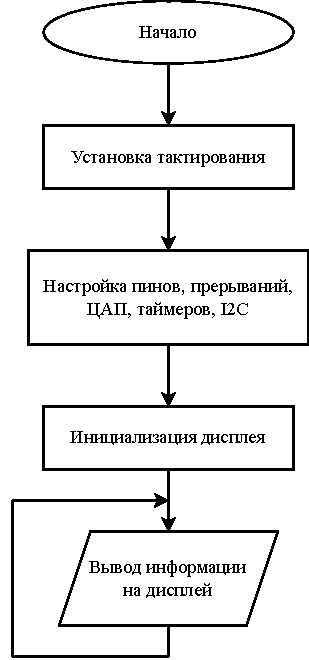
\includegraphics[width=0.36\textwidth]{../image/main.pdf}
    \caption{Блок-схема алгоритма главной функции.}
	\end{figure}
	
\begin{code}
\captionof{listing}{Главная функция программы}
\begin{minted}[mathescape,linenos,frame=lines,breaklines]{text}
int main(void)
{
    rcc_clock_setup_in_hse_8mhz_out_72mhz(); // установка тактирования
    gpio_setup();
    nvic_setup();
    dac_setup();
    timers_setup();
    i2c_setup();
    ssd1306_init(I2C2, DEFAULT_7bit_OLED_SLAVE_ADDRESS, 128, 64); // инициализация дисплея

    int f = 0;       // переменная частоты
    wchar_t freq[8]; // буфер для wchar_t строки
    while (1)
    {
        f = p_step / 24 * 125;
        swprintf(freq, sizeof(freq) / sizeof(wchar_t), L"%d", f); // Использование swprintf для преобразования int в wchar_t*
        /*  вывод информации на дисплей  */
        ssd1306_clear();
        ssd1306_drawWCharStr(0, 0, white, nowrap, L"Форма сигнала:");
        switch (num_sig)
        {
        case 1:
            ssd1306_drawWCharStr(0, 8, white, nowrap, L"Синус");
            break;
        ...
        case 5:
            ssd1306_drawWCharStr(0, 8, white, nowrap, L"Пила Правая");
            break;
        }
        ssd1306_drawWCharStr(0, 16, white, nowrap, L"Частота(Гц)");
        ssd1306_drawWCharStr(64, 16, white, nowrap, freq);
        ssd1306_drawWCharStr(0, 32, white, nowrap, L"Шаг(Гц)");
        switch (num_step)
        {
        case 1:
            ssd1306_drawWCharStr(64, 32, white, nowrap, L"125");
            break;
        ...
        case 4:
            ssd1306_drawWCharStr(64, 32, white, nowrap, L"1000");
            break;
        }
        ssd1306_refresh();
    }

    return 0;
}
\end{minted}
\end{code}
	
	Полный код программы содержится в приложении. После написания программы произведём сборку проекта и получим сообщение об успешной компиляции (рис. 2.11).
	
	\begin{figure}[H]
    \centering
    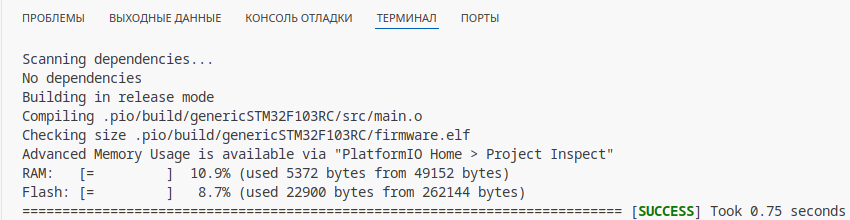
\includegraphics[width=0.825\textwidth]{../image/compile.png}
    \caption{Компиляция проекта.}
	\end{figure}
	
	Для более подробной информации проверим проект с помощью функции <<Inspect>>.
	
	\begin{figure}[H]
    \centering
    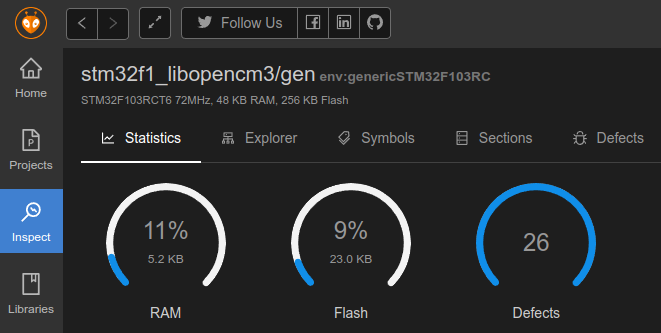
\includegraphics[width=0.8\textwidth]{../image/inspect.png}
    \caption{Проверка проекта.}
	\end{figure}
	
	Среда разработки описала занимаемую память и нашла дефекты в проекте.
	
	\begin{figure}[H]
    \centering
    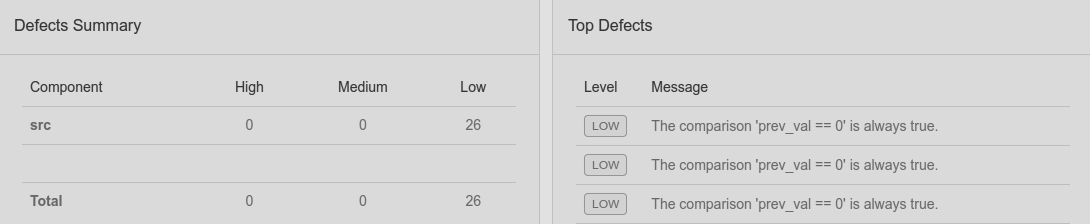
\includegraphics[width=1\textwidth]{../image/defects.png}
    \caption{Дефекты проекта.}
	\end{figure}
	
	Дефекты оказались незначительные и на работу программы влияния не оказывают.
	
\section{Вывод по второй главе}
	
	Таким образом, для реализации генератора сигналов был выбран микроконтроллер STM32F103RCT6 с использованием среды разработки PlatformIO и библиотеки libopencm3. Определен четкий план действий, включающий структуру программы, алгоритмы работы с цифро-аналоговым преобразователем, кнопками и дисплеем. Была разработана и скомпилирована результирующая программа, которая будет протестирована на макете устройства.

	
	
